% Final project for the completion of the bachelor's degree in Computer Engineering 
% at the "Enzo Ferrari" Department of Engineering at the University of Modena and Reggio Emilia

% 12-point font size
\documentclass[12pt]{report}

% Margins (2.5cm on all sides)
\usepackage[top=2.5cm, bottom=2.5cm, left=2.5cm, right=2.5cm, head=21.75pt, centering]{geometry}

% Line spacing
\linespread{1.5}
\usepackage[english]{babel} % applies writing rules for the English language
\usepackage[utf8]{inputenc} % UTF-8 encoding
\usepackage{scrlayer-scrpage} % page styles for the title page
\ifoot[]{}
\cfoot[]{}
\ofoot[\pagemark]{\pagemark}
\pagestyle{scrplain} 
\usepackage[hidelinks]{hyperref} % package for using hyperlinks
\usepackage[T1]{fontenc}
\usepackage{inconsolata}
\usepackage{newtxtext,newtxmath} % Times New Roman-like font
\usepackage{graphicx} % insertion of images
\usepackage{csquotes} % for block quotations
\usepackage{booktabs}    
\usepackage{adjustbox}  
\usepackage{filehook}
\usepackage{makecell}    
\usepackage{pifont}  
\usepackage[utf8]{inputenc} 
\usepackage[bottom]{footmisc}
\usepackage[T1]{fontenc} 
\usepackage[english]{babel}
\usepackage{graphicx} % insertion of images
\usepackage{subcaption} % for subfigures
\usepackage[backend=biber, sorting=nty]{biblatex} % bibliography using biblatex
\usepackage{verbatim} % to use \begin{comment} \end{comment}
\usepackage{multirow}
\appto{\bibsetup}{\raggedright}
\addbibresource{bibliography.bib} % links the bibliography file

\usepackage{titlesec} % for formatting section, chapter titles, etc.
\usepackage{float} % for positioning images

\usepackage{listings} % for programming code
\usepackage{color}
\usepackage{xurl}
\usepackage{tikz}
\usetikzlibrary{calc}
\usepackage{booktabs} % for \toprule, \midrule, \bottomrule in tables
\usepackage{algorithm}
\usepackage{algpseudocode}

% Definition of colors for code
\definecolor{lightgray}{rgb}{.9,.9,.9}
\definecolor{darkgray}{rgb}{.4,.4,.4}
\definecolor{purple}{rgb}{0.65, 0.12, 0.82}
\definecolor{mygreen}{rgb}{0,0.6,0}
\definecolor{mygray}{rgb}{0.5,0.5,0.5}
\definecolor{mymauve}{rgb}{0.58,0,0.82}
\definecolor{backcolour}{rgb}{0.95,0.95,0.92}

% Styles for programming languages
\lstdefinelanguage{JavaScript}{
  keywords={typeof, new, true, false, catch, function, return, null, catch, switch, var, let, const, if, in, while, do, else, case, break},
  keywordstyle=\color{blue}\bfseries,
  ndkeywords={class, export, boolean, throw, implements, import, this},
  ndkeywordstyle=\color{darkgray}\bfseries,
  identifierstyle=\color{black},
  sensitive=false,
  comment=[l]{//},
  morecomment=[s]{/*}{*/},
  morestring=[b]',
  morestring=[b]",
  commentstyle=\color{mygreen}\ttfamily,
  stringstyle=\color{mymauve}\ttfamily,
  backgroundcolor=\color{backcolour},
  basicstyle=\footnotesize\ttfamily,
  showstringspaces=false,
  extendedchars=true,
  showspaces=false,
  numbers=left,
  numberstyle=\footnotesize,
  numbersep=9pt,
  tabsize=2,
  breaklines=true,
  showtabs=false,
  captionpos=b
}

\lstdefinelanguage{MyPython}{
  language=Python,
  morekeywords={with, as},
  keywordstyle=\bfseries\color{blue},
  commentstyle=\color{mygreen},
  stringstyle=\color{mymauve},
  backgroundcolor=\color{backcolour},
  basicstyle=\footnotesize\ttfamily,
  showstringspaces=false,
  numbers=left,
  numberstyle=\footnotesize,
  numbersep=9pt,
  tabsize=2,
  breaklines=true,
  showtabs=false,
  captionpos=t
}

\lstdefinestyle{bash}{
    basicstyle=\ttfamily\small,
    rulesepcolor=\color{black},
    language=bash,
    breaklines=true,
    backgroundcolor=\color{backcolour},
    literate={"}{{\texttt{"}}}{1},
    numbers=left,
    numberstyle=\footnotesize,
    numbersep=9pt,
    columns=fixed,
    keepspaces=true,
}

\lstdefinestyle{Prompt}{
  breaklines=true,
  basicstyle=\ttfamily,
}

\lstdefinestyle{Myyaml}{
  basicstyle=\ttfamily\small,
  breaklines=true,
  numbers=left,
  numberstyle=\footnotesize,
  numbersep=9pt,
  showstringspaces=false,
  tabsize=2,
  backgroundcolor=\color{backcolour},
  columns=fixed,
  keepspaces=true,
}

% Format of headings
\titleformat{\chapter}[block]
  {\normalfont\LARGE\bfseries}{\thechapter.}{0.5em}{\LARGE}
\titlespacing*{\chapter}{0pt}{-20pt}{25pt}


\usepackage{enumitem}

\begin{document}

    \begin{titlepage}
         
    
        \begin{center}
            
\includegraphics[width=8cm]{images/unimore/Sigillo2015.png}
            \vspace{1cm}
    
            {\LARGE{ UNIVERSITY OF MODENA AND REGGIO EMILIA \\}}
            {\large{ "Enzo Ferrari" Department of Engineering \\}}
            % Comment and uncomment the right ones
            %{\large{ Master's Degree in Computer Engineering (LM-32) \\}} 
            {\large{ Master's Degree in Artificial Intelligence Engineering (LM-32) \\}}
            \vspace{3cm}
            {\Large { \textbf{Applying Explainability Methods to Financial Models} }}\\
            \vspace{3cm}
        \end{center}
        
        \begin{minipage}[t]{0.47\textwidth}
        	{\large{\bf Supervisor:}\\} 
        	{\large Prof. Francesco Guerra\\}
        \end{minipage}\hfill\begin{minipage}[t]{0.47\textwidth}\raggedleft
        	{\large{\bf Candidate:}\\}
            {\large Luca Villani}\\
            {\large Student ID 200412}
        \end{minipage}
        
        \vfill
        \hrulefill\\
        \centering{\large{\bf ACADEMIC YEAR 2024/2025}}
    \end{titlepage}
    
    \pagestyle{empty}
    \begin{flushright}
    \textit{<Dedication, optional. Delete everything on this page to remove it.>}
\end{flushright} 
    \clearpage
    
    \tableofcontents      % Generates the Table of Contents
    \renewcommand{\listfigurename}{List of Figures}
    \listoffigures        % Generates the List of Figures
    \renewcommand{\lstlistingname}{Code}
    \renewcommand{\lstlistlistingname}{List of Code}

    \lstlistoflistings    % Generates the List of Code Listings
    
    \clearpage
    \pagestyle{scrplain} % Restores the normal page style (with page number)
    \setcounter{page}{1} % Restart page numbering from 1

    % Add chapters here
    \chapter{Introduction}
\label{ch:introduction}

\section{Section}
\label{sec:objective}

This template can be used as a basis for writing the final thesis for the Master’s Degree in Computer Engineering/Artificial Intelligence Engineering. The table of contents, as well as the lists of figures and code listings, are generated automatically. The following chapter provides examples of basic elements.

\subsection{Subsection}
This is an example of a subsection.


    \chapter{Basic elements}
\label{ch:second_chapter}

This chapter will contain basic examples of bullet lists, figures, tables, formulas, algorithms, and code.

\bigskip
\noindent Example of a bullet list:
\begin{itemize}[noitemsep]
    \item \textbf{first bullet point in bold}; % in bold
    \item second bullet point, if you prefer it not to be in bold; % if you prefer it without bold
\end{itemize}

\section{Section in the Second Chapter}
\label{sec:id}

Example of an image in Figure \ref{fig:uno}. Remember to always reference in the text, using \textbackslash ref, all the figures/tables/algorithms/code you include.\footnote{An example of how to add a footnote, often used to cite or include a link to a website, such as~\url{https://ditto.ing.unimore.it/}\hspace{2pt}\raisebox{-0.4\height}{},}
    
\begin{figure}[H] % Starts the figure environment. [htbp] suggests placement: Here, Top, Bottom, Page.
    \centering % Centers the image and caption horizontally on the page.
    
    % \includegraphics[options]{filename} inserts the image.
    % --- Options ---
    % 'width=\linewidth': makes the image span the entire width of the text area.
    % Other options: 'width=8cm', 'scale=0.5' (half size),
    % 'height=5cm', 'angle=90' (rotate by 90 degrees).
    % 'keepaspectratio': prevents distortion when specifying both width and height.
    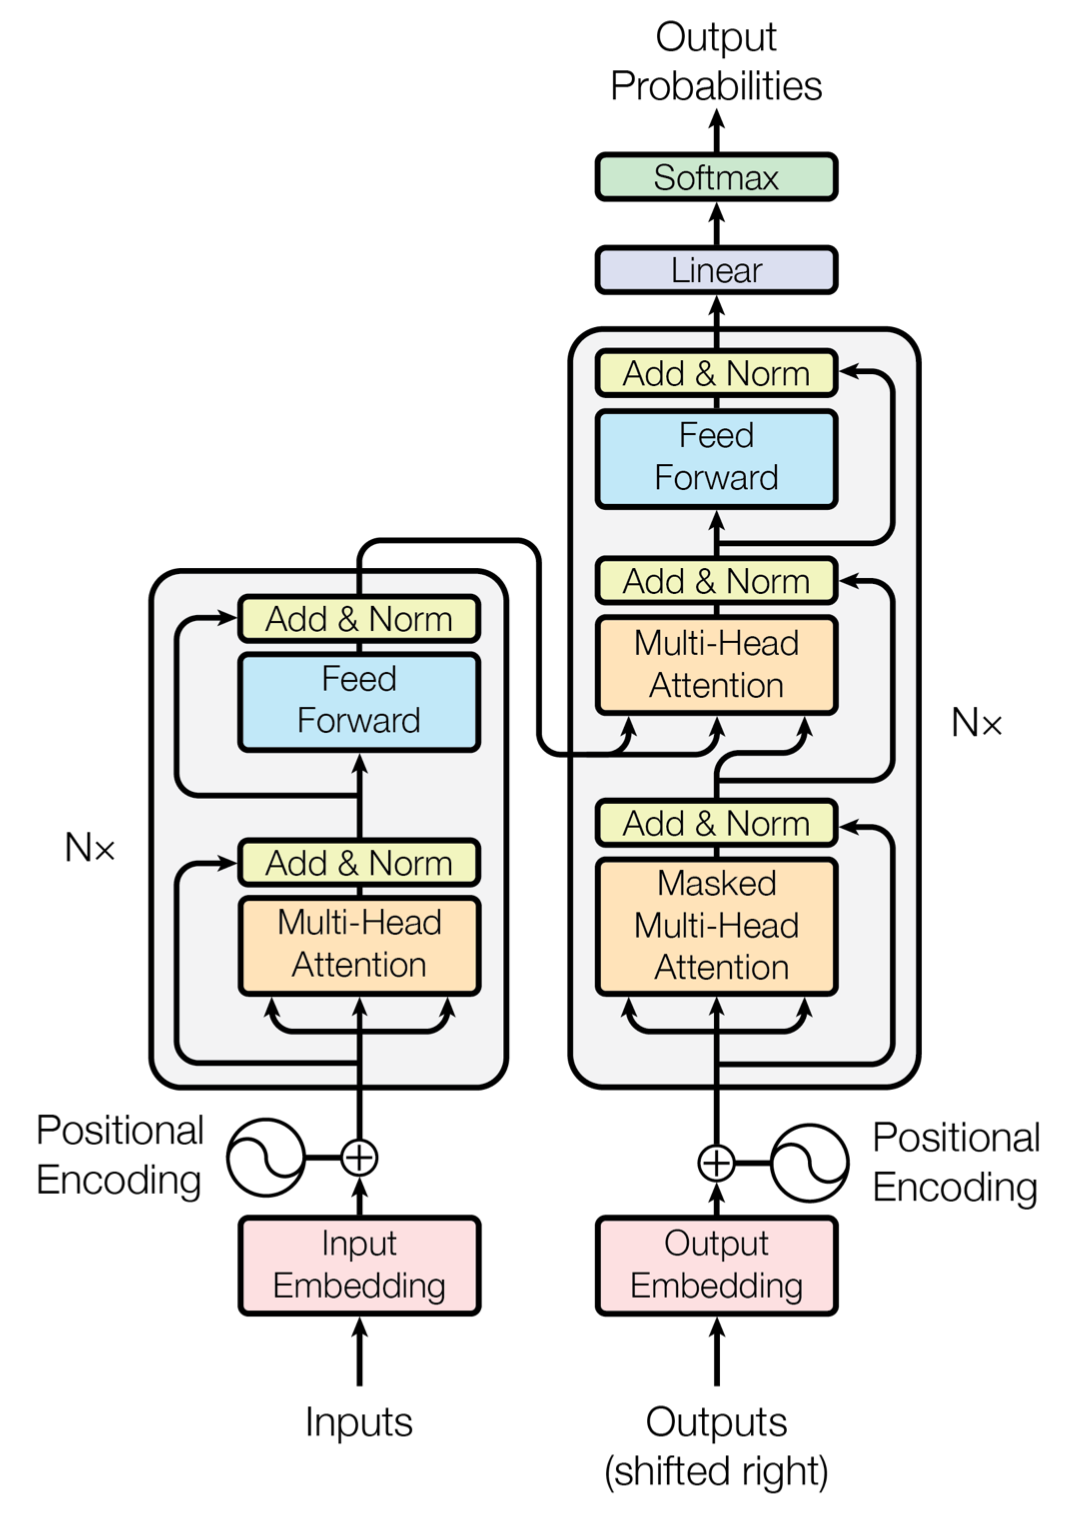
\includegraphics[width=0.8\linewidth, keepaspectratio]{images/architectures/t.png}
    
    \caption{The architecture introduced by Vaswani in the famous paper \textit{"Attention is All You Need"}~\cite{vaswani2017attention}.}
    \label{fig:uno}
\end{figure}

\section{Another Section in the Second Chapter}
Example of a table with its citation, Table~\ref{tab:table_example}.

\begin{table}[tb] % Start of floating table environment; [tb] = top or bottom of the page
\centering % Centers the table
\caption{Example of a table with various fields, checkmarks, and crosses.} % Caption
\begin{adjustbox}{width=0.9\textwidth} % Fits the table to 90% of the text width
{\normalsize % Sets normal font size
\setlength{\tabcolsep}{8pt} % Sets horizontal spacing between columns

\begin{tabular}{cccrrrr} % Creates a table with 7 columns:
                         % c = centered alignment, r = right alignment
\toprule % Thick upper horizontal rule (booktabs)

% \makecell allows formatted or multi-line text inside a cell.
% It is especially useful in headers to avoid using \parbox or \multicolumn.
% Here it is used to center and bold the header text.
\makecell[c]{\textbf{Fruit}} & 
\makecell[c]{\textbf{Orange-colored}} & 
\makecell[c]{\textbf{Peelable}} & 
\makecell[c]{\textbf{Weight}} &   
\makecell[c]{\textbf{Price}} &   
\makecell[c]{\textbf{Sugar}} &   
\makecell[c]{\textbf{Rating (1–10)}} \\  
% The symbol & separates columns within a row.
% Each cell of a row is delimited by an &.
% The \\ command ends the row and starts a new one.
\midrule % Medium horizontal rule

Orange & \checkmark  & \checkmark & 0.200 & 2.50 & 9.0 & 8 \\ % Example of a row: & separates columns, \\ closes the row
Mandarin & \checkmark & \checkmark & 0.120 & 3.20 & 8.5 & 9 \\
Lemon & \ding{55} & \checkmark & 0.100 & 3.50 & 2.5 & 6 \\
\midrule

Apple & \ding{55} & \ding{55} & 0.180 & 2.80 & 10.0 & 8 \\
Banana & \ding{55} & \checkmark & 0.150 & 1.10 & 12.2 & 9 \\
Kiwi & \ding{55} & \checkmark & 0.120 & 4.00 & 9.1 & 7 \\
Mango & \checkmark & \checkmark & 0.300 & 5.00 & 14.0 & 10 \\
\bottomrule % Thick lower horizontal rule

\end{tabular} % End of tabular environment
} % End of \normalsize block
\end{adjustbox} % End of width adjustment
\label{tab:table_example} % Label for referencing
\vspace{-10pt} % Reduces space below the table
\end{table} % End of table environment
 % input helps to keep the latex code cleaner by moving the table into another file

\section{Mathematical Formulas}
Here are two examples of how to write mathematical formulas. As you can easily recognize in Eq.~\ref{eq:continuous_ft}, we have the integral form of the Fourier Transform, while in Eq.~\ref{eq:discrete_ft} we see its discretized version using a summation.

% --- Formula 1: Continuous Fourier Transform (The Integral) ---
\begin{equation}
    \label{eq:continuous_ft}
    X(f) = \int_{-\infty}^{\infty} x(t) e^{-j 2\pi f t} \, dt
\end{equation}

% --- Formula 2: Discrete Fourier Transform (The Summation) ---
\begin{equation}
    \label{eq:discrete_ft}
    X_k = \sum_{n=0}^{N-1} x_n \cdot e^{-i \frac{2\pi}{N} k n}
\end{equation}

\section{Algorithm Example}
In Algorithm \ref{alg:dijkstra}, one way to compute the shortest path can be seen.

\begin{algorithm}[H] % H forces placement exactly here. Not recommended to always use it.
\caption{Dijkstra's Algorithm}
\label{alg:dijkstra}

    \begin{algorithmic}[1]
        
        \Procedure{Dijkstra}{$G, s$} 
            
            \State $dist[] \gets \infty$ \Comment{Initialize distances to infinity}
            \State $dist[s] \gets 0$     \Comment{Distance to the source is 0}
            \State $Q \gets V[G]$        \Comment{Add all nodes to the queue}
            
            \While{$Q$ is not empty} 
                \State $u \gets$ vertex in $Q$ with minimum $dist[u]$
                \State remove $u$ from $Q$
                
                \For{each neighbor $v$ of $u$} 
                    \State $alt \gets dist[u] + length(u, v)$
                    
                    \If{$alt < dist[v]$} 
                        \State $dist[v] \gets alt$
                        \State $prev[v] \gets u$
                    \EndIf
                    
                \EndFor
            \EndWhile
            
            \State \textbf{return} $dist[], prev[]$
            
        \EndProcedure 
        
    \end{algorithmic}
\end{algorithm}

\section{Code Examples}
You may also include some code samples, as long as they are not too long. An example can be seen in Code \ref{cod:hello}.

\begin{lstlisting}[caption={Example code, taken from helloworldspam.py}, label={cod:hello}]
print('Starting the ultimate hello world spammer')
for i in range(10000000):
    print("Hello, world!")
\end{lstlisting}

\section{Bibliography Management}
All bibliographic references must be inserted into the project’s ``.bib'' file. In this template, the file is ``bibliography.bib''. To cite a reference, use the command ``\textbackslash cite\{<id>\}'', such as \cite{vaswani2017attention}.

    
    \chapter{Tables and Images}
\label{ch:third_chapter}
This chapter contains examples of large tables and grid-arranged images.

\section{1x3 Grid}
Here is an example of an image grid, as shown in Figure \ref{fig:fruit_images1x3}.
\begin{figure}[h!]
\centering

\begin{subfigure}[t]{0.30\textwidth}
  \centering
  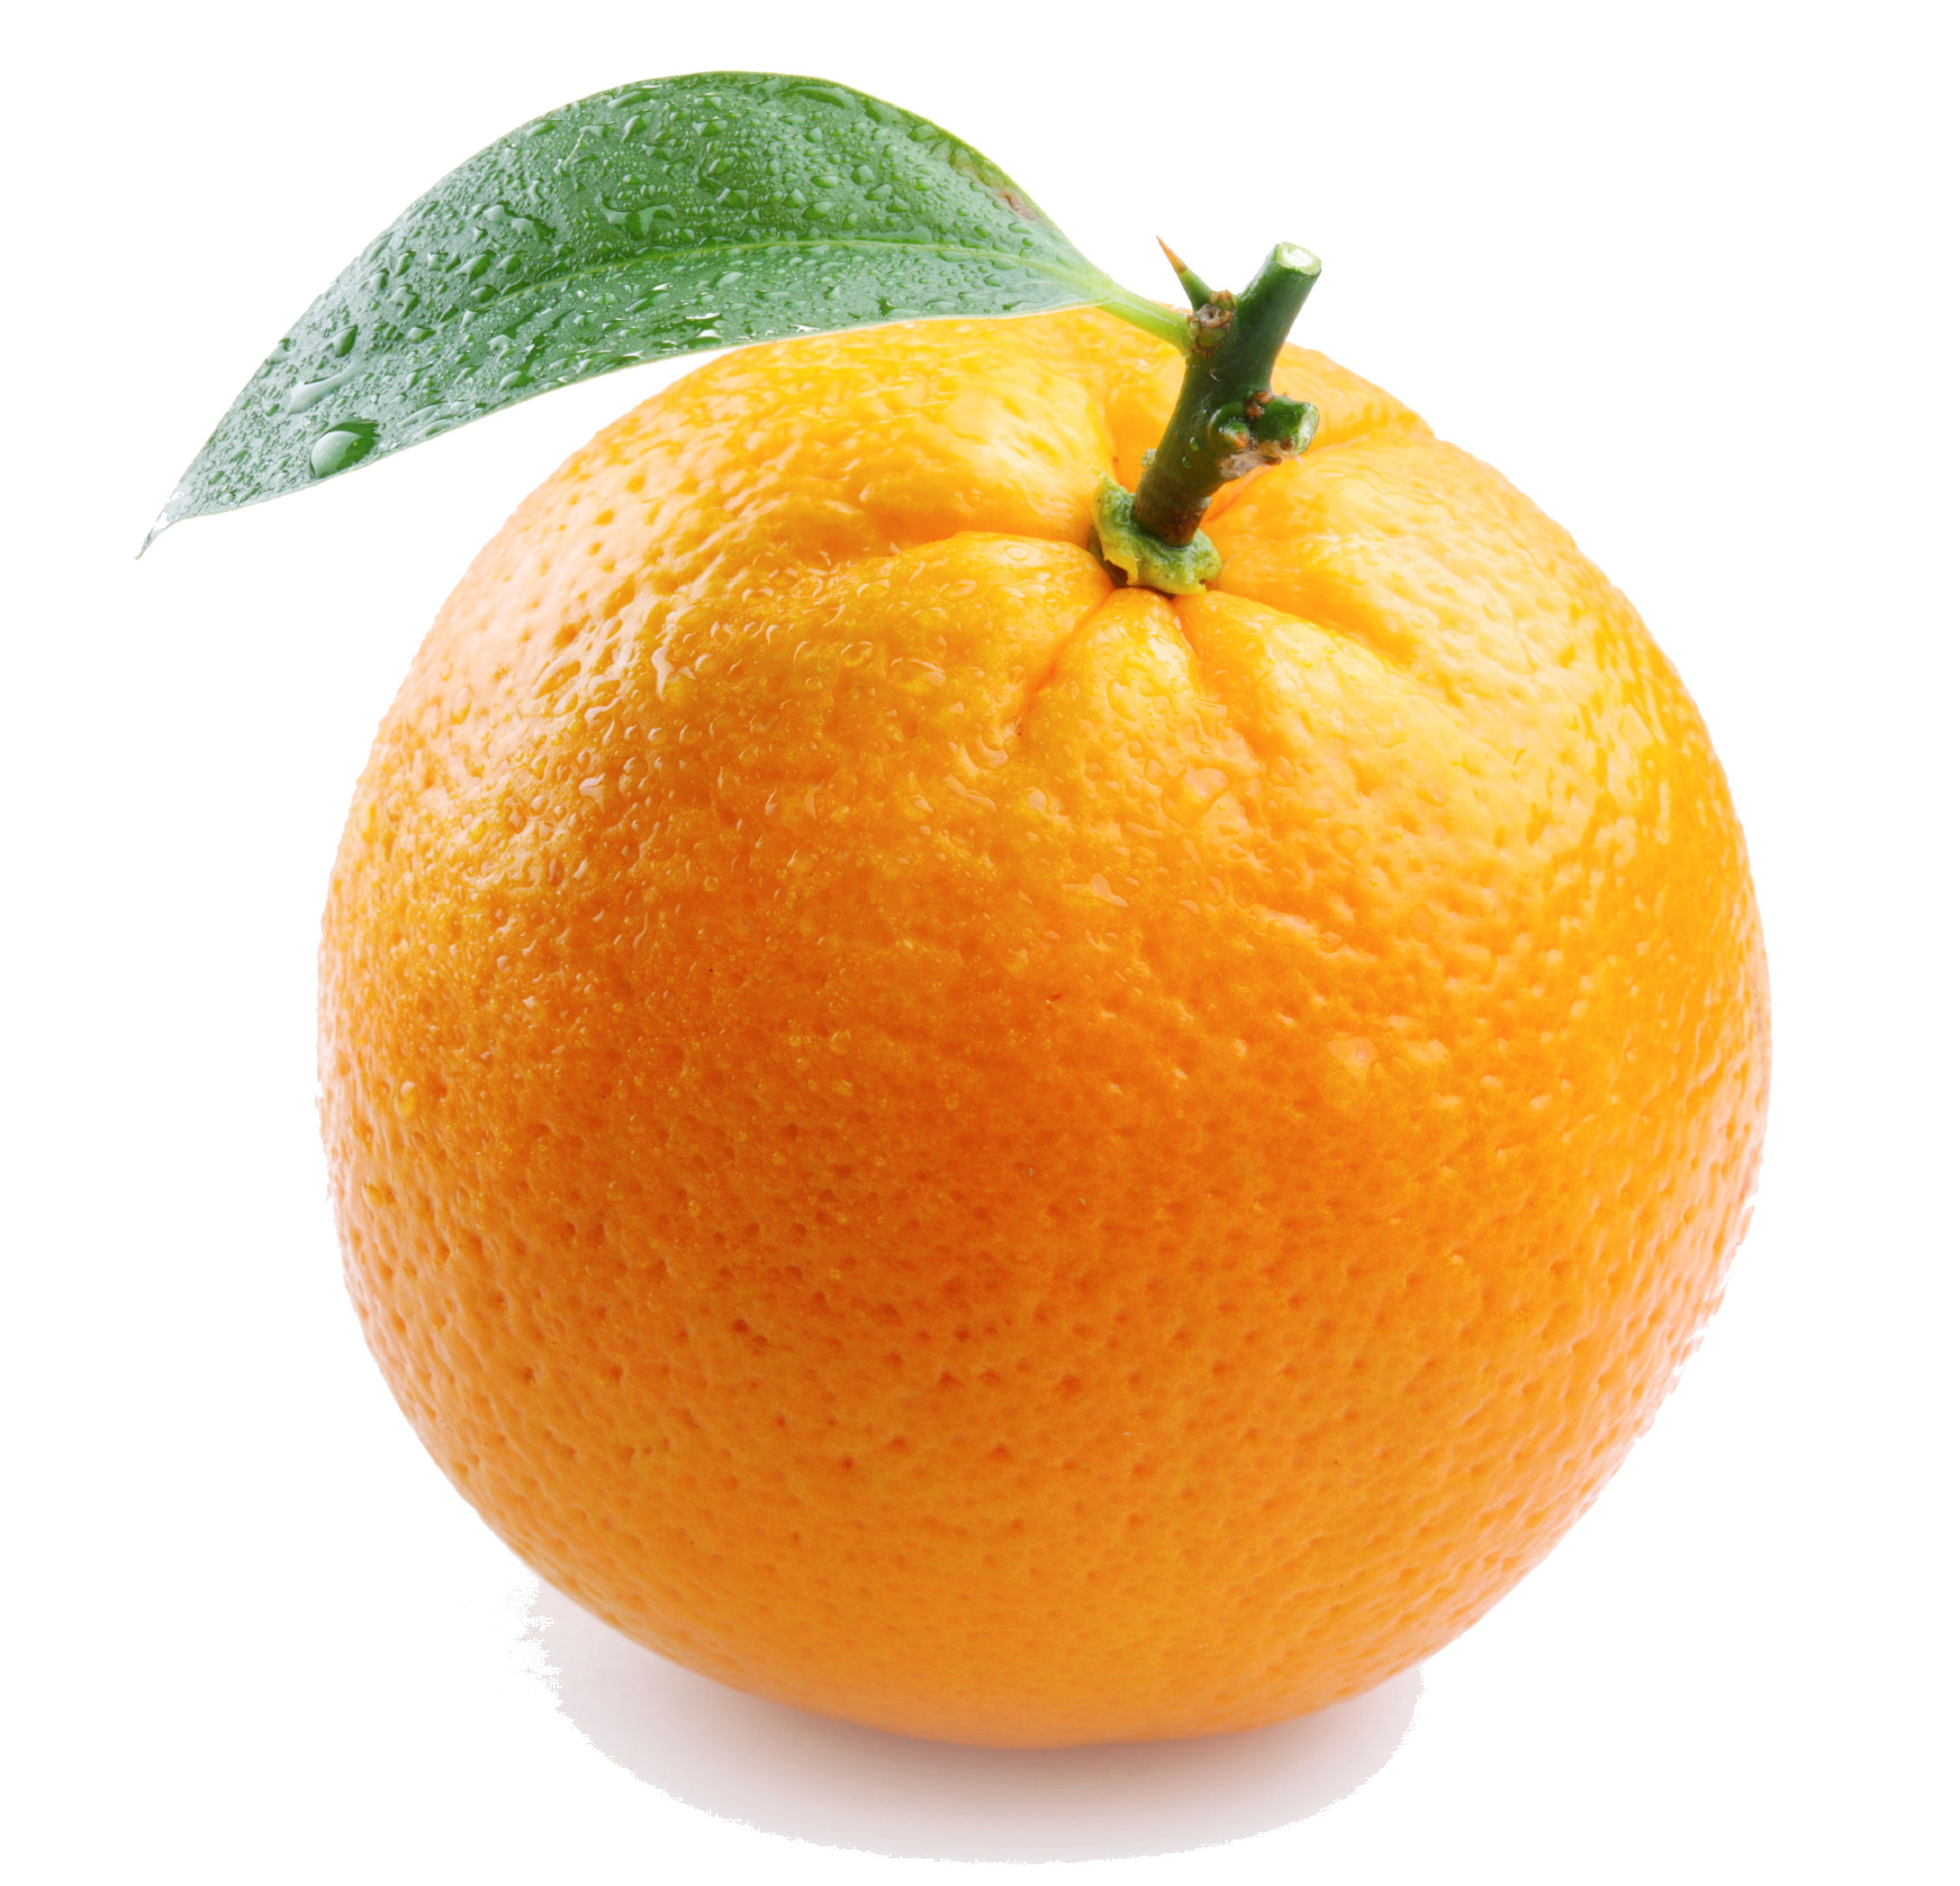
\includegraphics[width=\linewidth]{images/fruits/arancia.jpg}
  \caption{Orange}
\end{subfigure}\hfill
\begin{subfigure}[t]{0.30\textwidth}
  \centering
  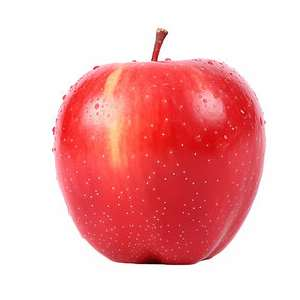
\includegraphics[width=\linewidth]{images/fruits/mela.jpg}
  \caption{Apple}
\end{subfigure}\hfill
\begin{subfigure}[t]{0.30\textwidth}
  \centering
  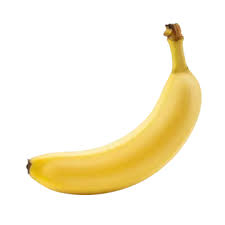
\includegraphics[width=\linewidth]{images/fruits/banana.jpg}
  \caption{Banana}
\end{subfigure}

\caption{Photos of fresh fruit in a 1x3 grid.}
\label{fig:fruit_images1x3}
\end{figure}

\section{2x2 Grid}
Here is an example of an image grid, as shown in Figure \ref{fig:fruit_images2x2}.
\begin{figure}[H]
\centering

% --- First row ---
\begin{subfigure}[t]{0.45\textwidth}
  \centering
  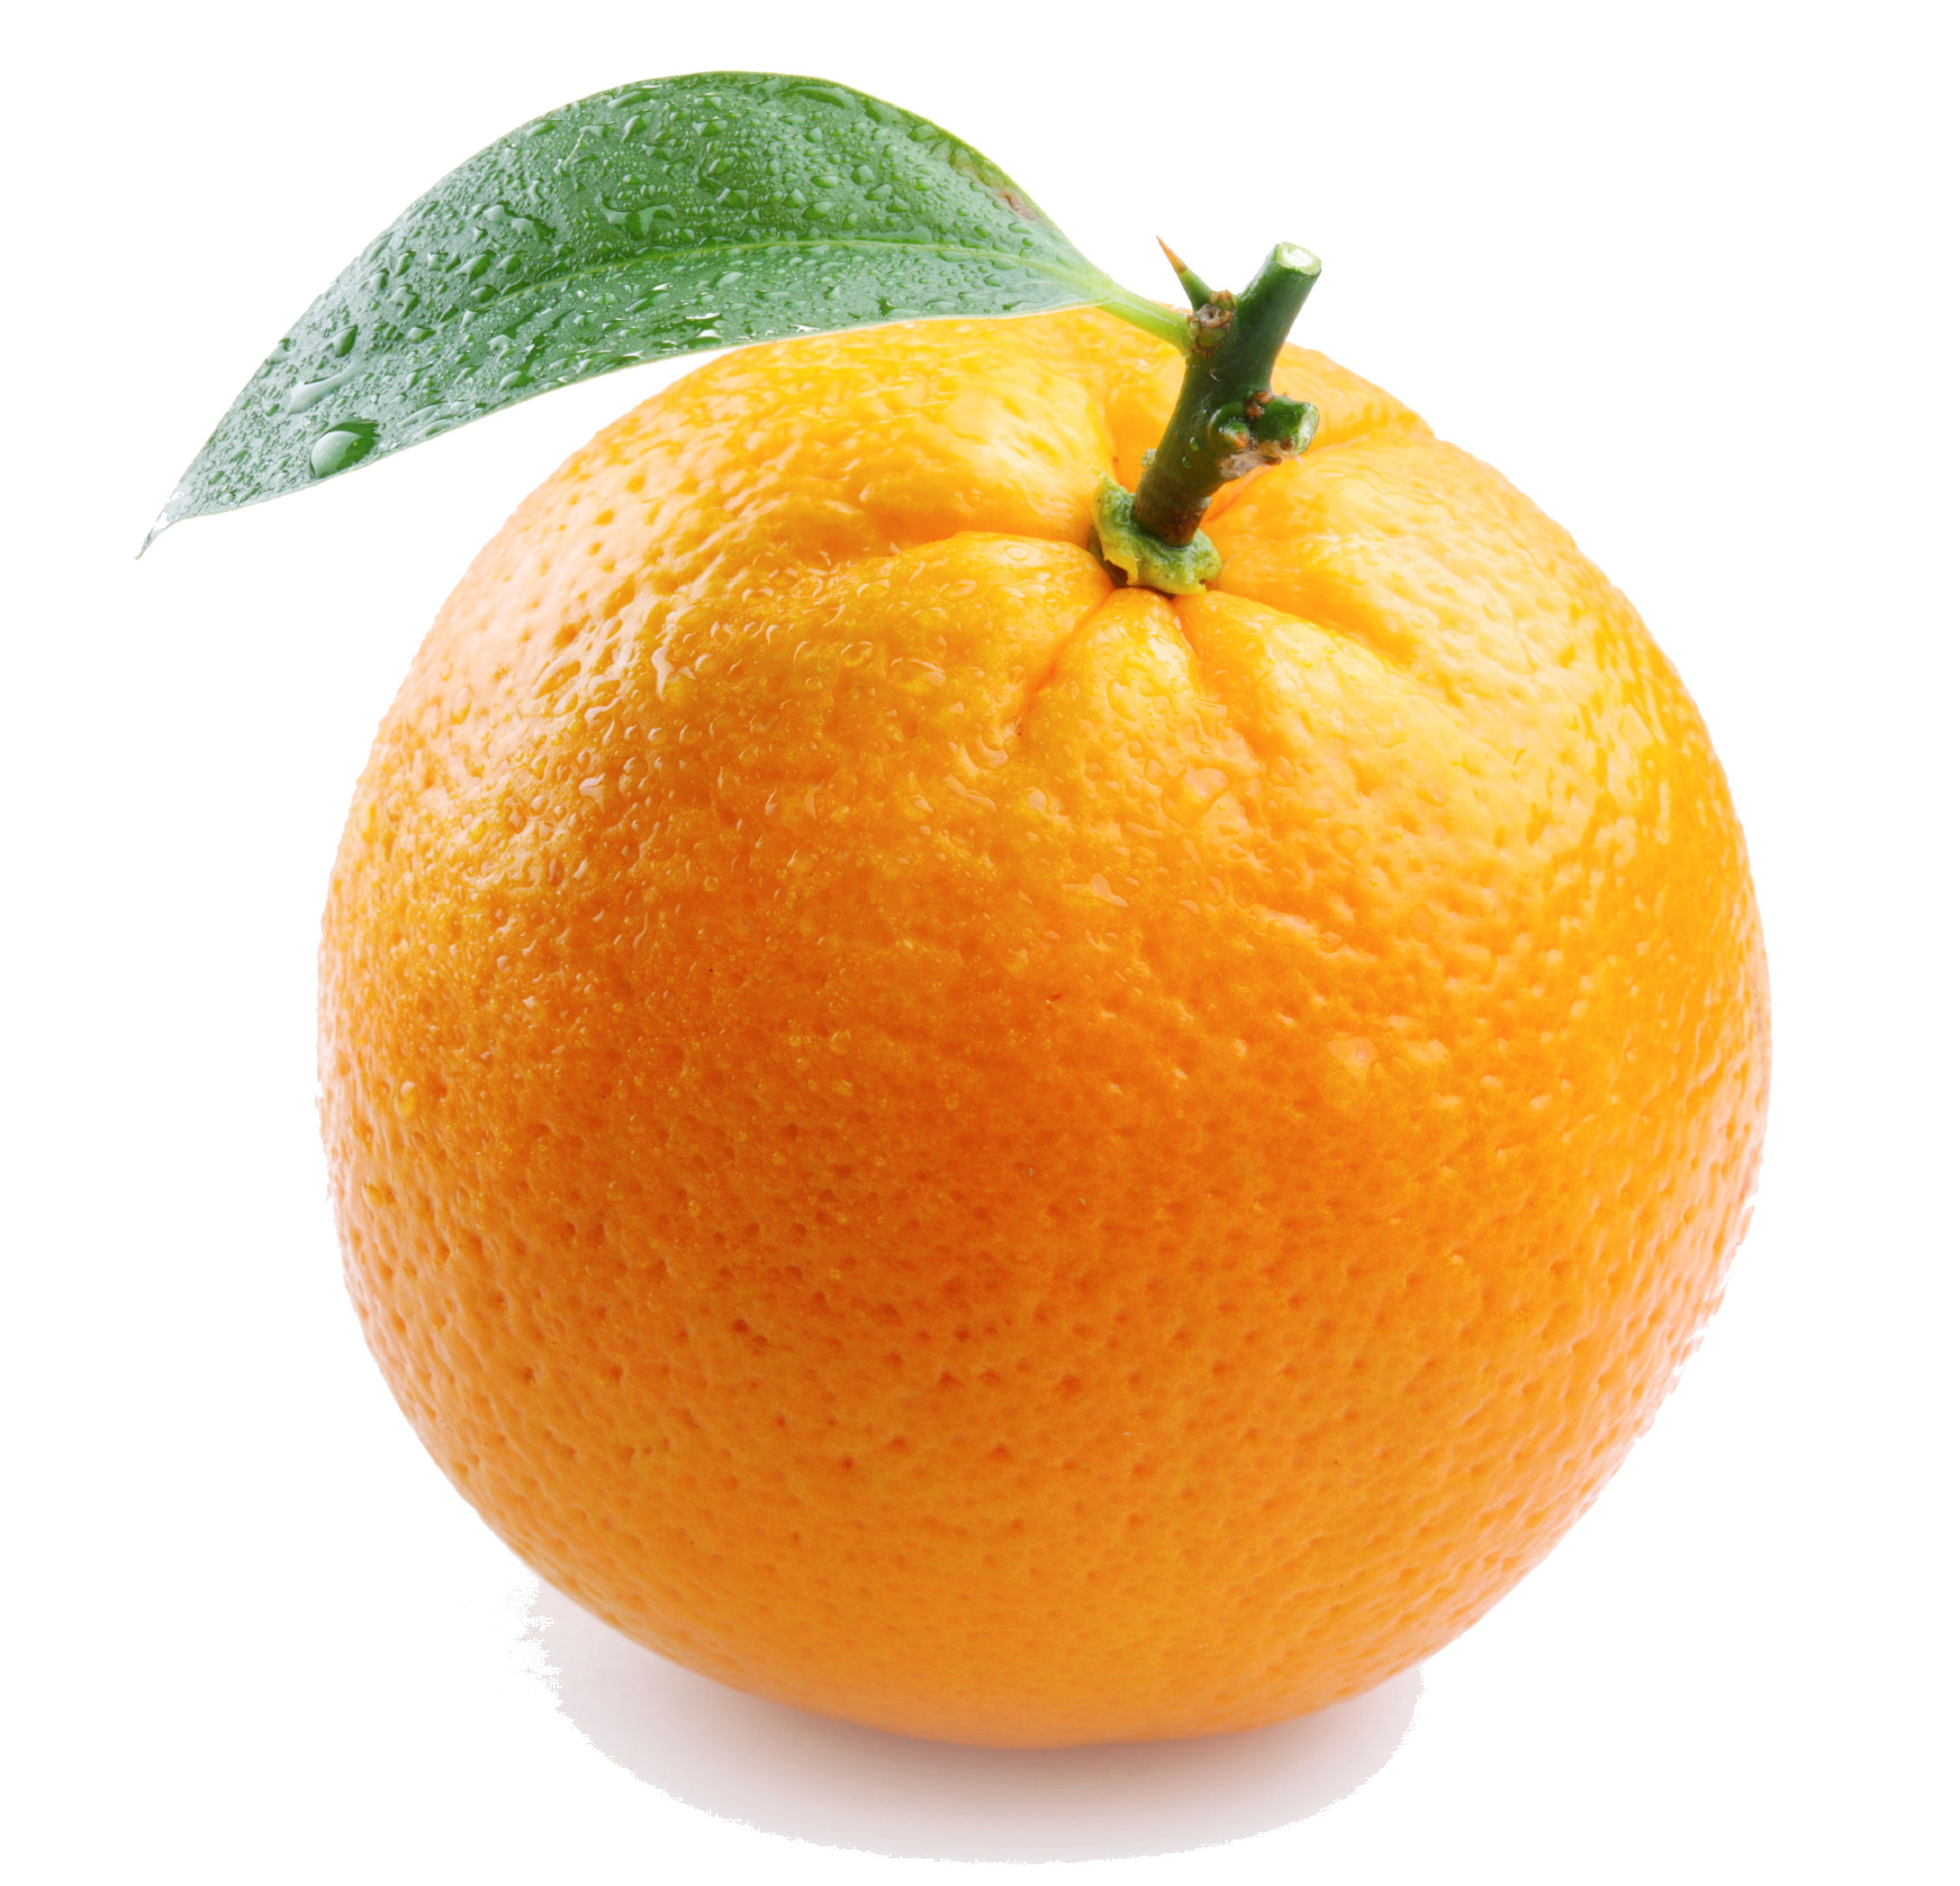
\includegraphics[width=\linewidth]{images/fruits/arancia.jpg}
  \caption{Orange}
\end{subfigure}\hfill
\begin{subfigure}[t]{0.45\textwidth}
  \centering
  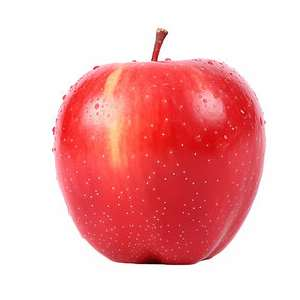
\includegraphics[width=\linewidth]{images/fruits/mela.jpg}
  \caption{Apple}
\end{subfigure}

% --- Second row ---
\begin{subfigure}[t]{0.45\textwidth}
  \centering
  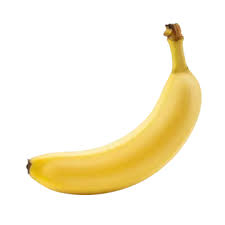
\includegraphics[width=\linewidth]{images/fruits/banana.jpg}
  \caption{Banana}
\end{subfigure}\hfill
\begin{subfigure}[t]{0.45\textwidth}
  \centering
  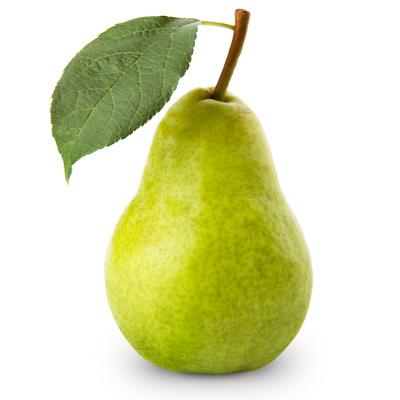
\includegraphics[width=\linewidth]{images/fruits/pera.jpg}
  \caption{Pear}
\end{subfigure}

\caption{Photos of fresh fruit in a 2×2 grid.}
\label{fig:fruit_images2x2}
\end{figure}

\section{Example of a Complex Table}
\input{tables/complex_table}

    
    Chapter{Conclusions}
\label{ch:conclusions}

Your conclusions would go here.

    \chapter*{Acknowledgements}
\addcontentsline{toc}{chapter}{Acknowledgements}

Here you may include your acknowledgements (ringraziamenti), if you wish.
    
    \clearpage 
    
    \addcontentsline{toc}{chapter}{References}
    
    \printbibliography[heading=subbibliography, title=Bibliography]

    \nocite{*}
   
\end{document}
